\documentclass{article}
\usepackage[top=2.5cm, left=3cm, right=3cm, bottom=4.0cm]{geometry}
\usepackage{graphicx} 
\usepackage{amsfonts,amsmath,amssymb}
\usepackage{array}
\usepackage{tabularray}
\usepackage[utf8]{inputenc}
\usepackage[T1]{fontenc}
\usepackage{csquotes}
\usepackage{alphabeta}
\usepackage{url}
\usepackage{hyperref}
\usepackage{esint}

\renewcommand{\figurename}{Γράφημα}

\begin{document}
\begin{table}[ht]
    \begin{tblr}{
        @{}X[l, valign=b]X[c, valign=b]X[r, valign=b]@{}
    }

    \hline
    % First line, course info
    \SetCell[c=2]{l}{[ΘΠ04] Παράλληλα Συστήματα} & & {2024-25} \\ 
    \hline
    {} & {} & {} \\

    % Title
    \SetCell[c=3]{c}{ \Large \textbf{Εργασία 3 - Προγραμματισμός με MPI} } \\
    {} & {} & {} \\

    % Name Surname, Student ID
    \hline
    \SetCell[c=3]{c}{ \textbf{Ονοματεπώνυμο:} Μάριος Γιαννόπουλος } \\
    \SetCell[c=3]{c}{ \textbf{A.M.:} 1115200000032} \\
    \hline

    \end{tblr}
\end{table}
\section*{Γενικές Πληροφορίες}

\subsection*{Υπολογιστικό Σύστημα}
Όλο το έργο υλοποιήθηκε στο ίδιο υπολογιστικό περιβάλλον:
\begin{itemize}
    \item \textbf{Όνομα Υπολογιστικού Συστήματος:} Linux12
    \item \textbf{Επεξεργαστής:} Intel(R) Core(TM) i5-6500 CPU @ 3.20GHz
    \item \textbf{Αριθμός Πυρήνων:} 4
    \item \textbf{Λειτουργικό Σύστημα:} Linux Ubuntu 20.04.2 LTS
    \item \textbf{Έκδοση Μεταγλωττιστή:} gcc (Ubuntu 9.4.0-1ubuntu1~20.04.2) 9.4.0
\end{itemize}

\subsection*{Οδηγίες Εκτέλεσης Python Scripts}
Για την εκτέλεση των Python scripts που επεξεργάζονται τα αποτελέσματα, ακολουθήστε τα εξής βήματα:
\begin{enumerate}
    \item Μεταβείτε στον φάκελο \path{scripts}.
    \item Εγκαταστήστε τις απαραίτητες βιβλιοθήκες:
    \begin{verbatim}
    pip install -r requirements.txt
    \end{verbatim}
    \item Εκτελέστε το script που σας ενδιαφέρει:
    \begin{verbatim}
    python <test_script>.py
    \end{verbatim}
\end{enumerate}
\textbf{Σημείωση:} Όλα τα αποτελέσματα στα γραφήματα είναι από την εκτέλεση των πειραμάτων στο εργαστήριο Linux. Κάθε πείραμα εκτελέστηκε 5 φορές και τα αποτελέσματα αναφέρονται στο μέσο όρο των επαναλήψεων.
\section*{Άσκηση 3.1}
\subsection*{Εισαγωγή}
Το Παιχνίδι της Ζωής (Game of Life) είναι ένα κυτταρικό αυτόματο που αναπτύχθηκε από τον μαθηματικό John Horton Conway. Είναι ένα μοντέλο που προσομοιώνει την εξέλιξη ενός πληθυσμού κυττάρων σε ένα δισδιάστατο πλέγμα, όπου κάθε κύτταρο μπορεί να βρίσκεται σε μία από δύο καταστάσεις: ζωντανό ή νεκρό. 
Οι κανόνες που διέπουν την εξέλιξη του πληθυσμού βασίζονται στον αριθμό των γειτόνων κάθε κυττάρου.
Σε αυτή την άσκηση, υλοποιήθηκε μια παράλληλη έκδοση του Παιχνιδιού της Ζωής χρησιμοποιώντας την MPI (Message Passing Interface) για την κατανομή του υπολογιστικού φόρτου μεταξύ πολλαπλών διεργασιών. Η υλοποίηση βασίζεται στη σειριακή έκδοση του αλγορίθμου που αναπτύχθηκε στην Άσκηση 2.1, χωρίς τη χρήση OpenMP.
\subsection*{Συγχρονισμός}
Ο συγχρονισμός μεταξύ των διεργασιών είναι ένα κρίσιμο στοιχείο στην παράλληλη υλοποίηση του Παιχνιδιού της Ζωής. Στον κώδικα, ο συγχρονισμός επιτυγχάνεται με τις εξής λειτουργίες:
\begin{enumerate}
    \item \textbf{\path{MPI_Scatter}}: Η διεργασία 0 κατανέμει τα δεδομένα του πλέγματος στις υπόλοιπες διεργασίες.
    \item \textbf{\path{MPI_Sendrecv}}: Κάθε διεργασία ανταλλάσσει γραμμές ορίων (ghost rows) με τις γειτονικές της διεργασίες για να υπολογίσει σωστά την επόμενη γενιά.
    \item \textbf{\path{MPI_Gather}}: Η διεργασία 0 συγκεντρώνει τα αποτελέσματα από όλες τις διεργασίες για να ενημερώσει το τελικό πλέγμα.
    \item \textbf{\path{MPI_Barrier}}: Εξασφαλίζει ότι όλες οι διεργασίες έχουν ολοκληρώσει την τρέχουσα γενιά πριν προχωρήσουν στην επόμενη.
\end{enumerate}
Αυτές οι λειτουργίες εξασφαλίζουν ότι οι διεργασίες συνεργάζονται αποτελεσματικά και ότι τα δεδομένα παραμένουν συνεπή κατά τη διάρκεια της εκτέλεσης.
\subsection*{Πειραματική Διαδικασία}
\begin{itemize}
    \item \textbf{Παραμετροποίηση:}
    \begin{itemize}
        \item Μέγεθος πλέγματος: $64 \times 64$, $1024 \times 1024$, $4096 \times 4096$.
        \item Αριθμός γενιών: 1000.
    \end{itemize}
    \item \textbf{Εκτέλεση:}
    \begin{itemize}
        \item Τα πειράματα εκτελέστηκαν 5 φορές για κάθε συνδυασμό παραμέτρων.
        \item Καταγράφηκε ο χρόνος εκτέλεσης για κάθε πείραμα.
        \item Τα δεδομένα αποθηκεύτηκαν σε CSV αρχείο.
    \end{itemize}
    \item \textbf{Αυτοματοποίηση:}
    \begin{itemize}
        \item Αναπτύχθηκαν Python scripts για την εκτέλεση των πειραμάτων και την καταγραφή των δεδομένων.
        \item Χρησιμοποιήθηκαν Python scripts για την επεξεργασία των αποτελεσμάτων και τη δημιουργία γραφημάτων.
    \end{itemize}
\end{itemize}
\subsection*{Αποτελέσματα}
Από τα αποτελέσματα των μετρήσεων, παρατηρούμε τα εξής:
\begin{enumerate}
    \item \textbf{Για μικρά μεγέθη πλέγματος (64x64)}:
    \begin{itemize}
        \item Η χρήση περισσότερων διεργασιών δεν οδηγεί πάντα σε μείωση του χρόνου εκτέλεσης. Για παράδειγμα, η χρήση 4 διεργασιών οδήγησε σε μεγαλύτερο χρόνο εκτέλεσης (2.20885 s) σε σύγκριση με τη χρήση 2 διεργασιών (1.72495 s). Αυτό οφείλεται στο γεγονός ότι το κόστος επικοινωνίας μεταξύ των διεργασιών είναι υψηλό σε σχέση με τον χρόνο υπολογισμού για τόσο μικρά πλέγματα.
        \item Η χρήση 8 και 16 διεργασιών οδήγησε σε ακόμη μεγαλύτερους χρόνους εκτέλεσης (7.92210 s και 10.79159 s αντίστοιχα), γεγονός που επιβεβαιώνει ότι για μικρά πλέγματα η παράλληλη εκτέλεση δεν είναι αποτελεσματική.
    \end{itemize}
    \item \textbf{Για μεσαία μεγέθη πλέγματος (1024x1024)}:
    \begin{itemize}
        \item Η χρήση 4 διεργασιών οδήγησε σε σημαντική μείωση του χρόνου εκτέλεσης (7.71714 s) σε σύγκριση με τη χρήση 2 διεργασιών (21.93556 s). Αυτό δείχνει ότι για μεσαία μεγέθη πλέγματος, η παράλληλη εκτέλεση αρχίζει να γίνεται αποτελεσματική.
        \item Ωστόσο, η χρήση 8 και 16 διεργασιών οδήγησε σε αύξηση του χρόνου εκτέλεσης (22.11091 s και 16.76202 s αντίστοιχα), γεγονός που υποδηλώνει ότι το κόστος επικοινωνίας αρχίζει να γίνεται σημαντικό για μεγαλύτερο αριθμό διεργασιών.
    \end{itemize}
    \item \textbf{Για μεγάλα μεγέθη πλέγματος (4096x4096)}:
    \begin{itemize}
        \item Η χρήση περισσότερων διεργασιών οδήγησε σε σημαντική μείωση του χρόνου εκτέλεσης. Για παράδειγμα, η χρήση 16 διεργασιών οδήγησε σε μέσο χρόνο εκτέλεσης 75.97231 s, σε σύγκριση με 425.03920 s για 2 διεργασίες.
        \item Αυτό δείχνει ότι για πολύ μεγάλα πλέγματα, η παράλληλη εκτέλεση είναι πολύ αποτελεσματική, καθώς ο χρόνος υπολογισμού κυριαρχεί έναντι του χρόνου επικοινωνίας.
    \end{itemize}
\end{enumerate}
\subsection*{Γραφήματα}
\begin{figure}[h]
    \centering
    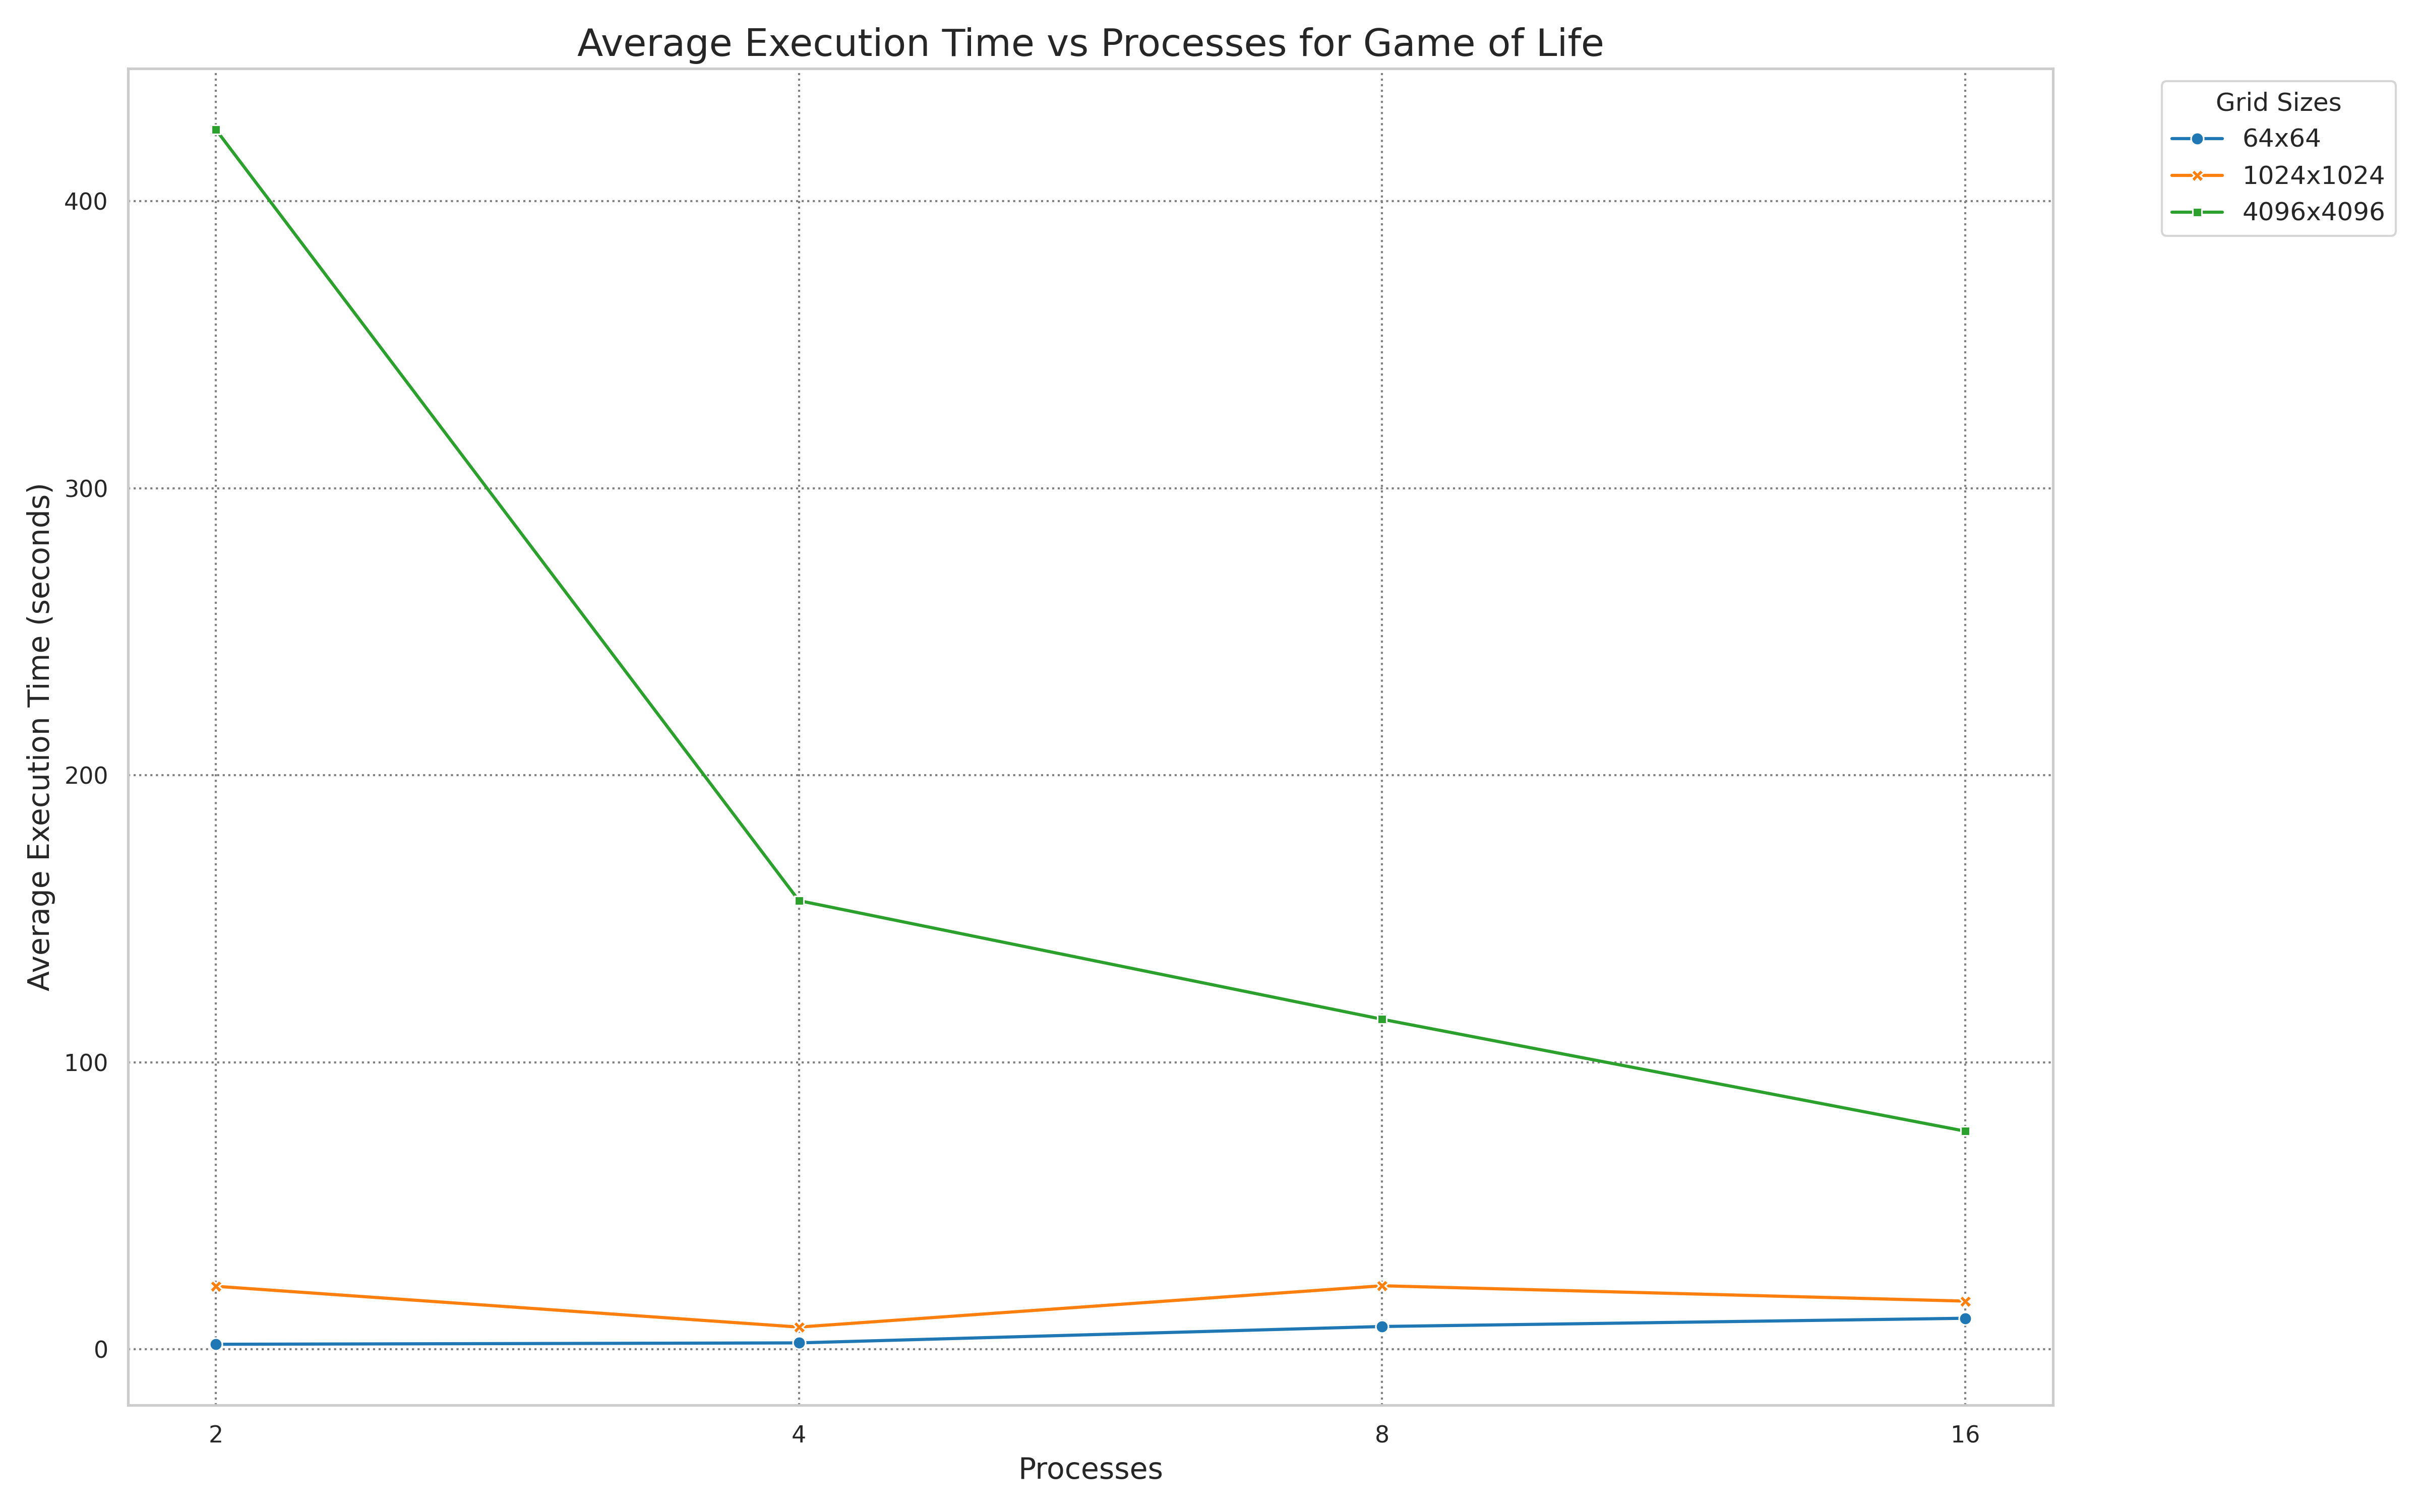
\includegraphics[width=0.8\textwidth]{game_of_life_mpi_results.png}
    \caption{Χρόνοι εκτέλεσης για το Παιχνίδι της Ζωής με MPI}
\end{figure}
\subsection*{Συμπεράσματα}
Από τα αποτελέσματα και τα γραφήματα, μπορούμε να εξάγουμε τα εξής συμπεράσματα:
\begin{enumerate}
    \item \textbf{Επίδραση του μεγέθους πλέγματος}:
    \begin{itemize}
        \item Για μικρά μεγέθη πλέγματος, η παράλληλη εκτέλεση δεν είναι αποτελεσματική λόγω του υψηλού κόστους επικοινωνίας σε σχέση με τον χρόνο υπολογισμού.
        \item Για μεσαία και μεγάλα μεγέθη πλέγματος, η παράλληλη εκτέλεση γίνεται ολοένα και πιο αποτελεσματική, καθώς ο χρόνος υπολογισμού κυριαρχεί έναντι του χρόνου επικοινωνίας.
    \end{itemize}
    \item \textbf{Επίδραση του αριθμού των διεργασιών}:
    \begin{itemize}
        \item Για μικρά πλέγματα, η αύξηση του αριθμού των διεργασιών οδηγεί σε αύξηση του χρόνου εκτέλεσης λόγω του κόστους επικοινωνίας.
        \item Για μεγάλα πλέγματα, η αύξηση του αριθμού των διεργασιών οδηγεί σε σημαντική μείωση του χρόνου εκτέλεσης, καθώς ο χρόνος υπολογισμού είναι πολύ μεγαλύτερος από το κόστος επικοινωνίας.
    \end{itemize}
    \item \textbf{Βέλτιστος αριθμός διεργασιών}:
    \begin{itemize}
        \item Για κάθε μέγεθος πλέγματος, υπάρχει ένας βέλτιστος αριθμός διεργασιών που εξαρτάται από το μέγεθος του πλέγματος και το κόστος επικοινωνίας. Για παράδειγμα, για πλέγμα 1024x1024, ο βέλτιστος αριθμός διεργασιών φαίνεται να είναι 4, ενώ για πλέγμα 4096x4096, ο βέλτιστος αριθμός διεργασιών φαίνεται να είναι 16.
    \end{itemize}
\end{enumerate}
Συνολικά, η παράλληλη υλοποίηση του Παιχνιδιού της Ζωής με MPI αποδεικνύεται πολύ αποτελεσματική για μεγάλα προβλήματα, ενώ για μικρά προβλήματα η σειριακή εκτέλεση μπορεί να είναι επαρκής. Η επιλογή του βέλτιστου αριθμού διεργασιών εξαρτάται από το μέγεθος του πλέγματος και το κόστος επικοινωνίας μεταξύ των διεργασιών.
\section*{Άσκηση 3.2}
\subsection*{Εισαγωγή}
\subsection*{Πειραματική Διαδικασία}
\subsection*{Αποτελέσματα}
\subsection*{Γραφήματα}
\subsection*{Συμπεράσματα}
\section*{Άσκηση 3.3}
\subsection*{Εισαγωγή}
\subsection*{Πειραματική Διαδικασία}
\subsection*{Αποτελέσματα}
\subsection*{Γραφήματα}
\subsection*{Συμπεράσματα}
\section*{Άσκηση 3.4}
\subsection*{Εισαγωγή}
\subsection*{Πειραματική Διαδικασία}
\subsection*{Αποτελέσματα}
\subsection*{Γραφήματα}
\subsection*{Συμπεράσματα}
\end{document}